\section{Sandbox}

\subsection{Images}

\subsubsection{Just an image}

\begin{center}
    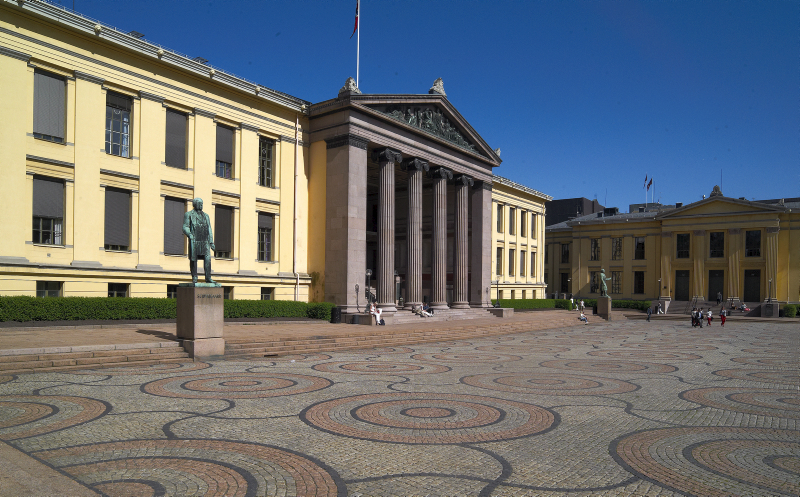
\includegraphics[width=0.7\columnwidth]{./img/university-square-uio.jpg}
\end{center}

\subsubsection{Proper figure}

\begin{figure}[ht]
    \centering
    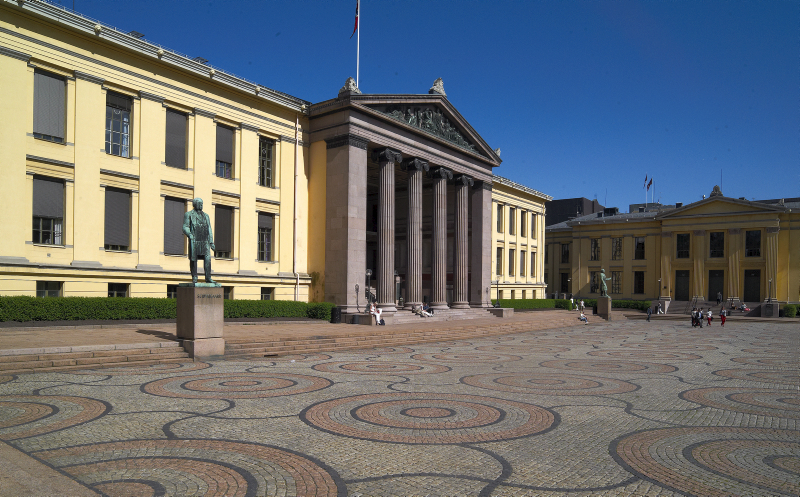
\includegraphics[width=0.7\textwidth]{./img/university-square-uio.jpg}
    \caption{UiO university, some text, some more text, and some other things just to make this multi-line and super long text, to demonstrate how a different style applies to figure captions}
    \label{fig:uio-university}
\end{figure}

\subsubsection{Figure with wrapping text}

\begin{wrapfigure}{R}{0.6\textwidth}
    \begin{center}
        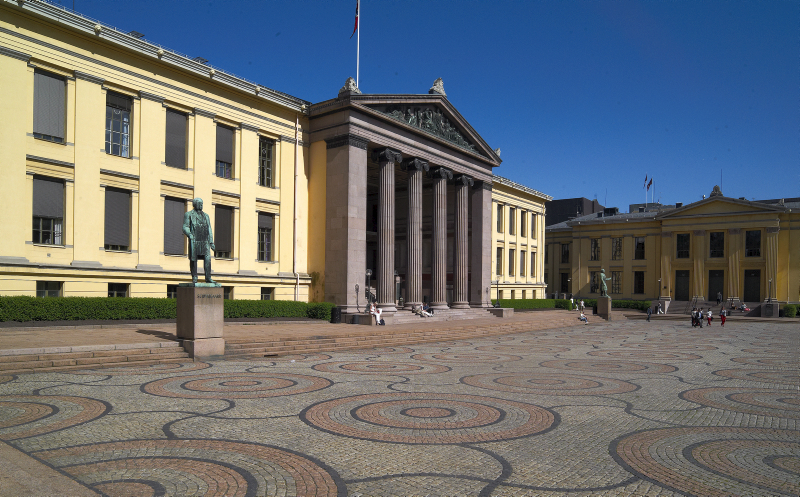
\includegraphics[width=0.6\textwidth]{./img/university-square-uio.jpg}
    \end{center}
    \caption{UiO university, some text, some more text, and some other things just to make this multi-line and super long text, to demonstrate how a different style applies to figure captions}
\end{wrapfigure}

Lorem ipsum dolor sit amet, consectetur adipisicing elit, sed do eiusmod tempor incididunt ut labore et dolore magna aliqua. Ut enim ad minim veniam.

Lorem ipsum dolor sit amet, consectetur adipisicing elit, sed do eiusmod tempor incididunt ut labore et dolore magna aliqua. Ut enim ad minim veniam, quis nostrud exercitation ullamco laboris nisi ut aliquip ex ea commodo consequat. Duis aute irure dolor in reprehenderit in voluptate velit esse cillum dolore eu fugiat nulla pariatur. Excepteur sint occaecat cupidatat non proident, sunt in culpa qui officia deserunt mollit anim id est laborum.

\subsection{Formulas}
\label{sec:frmls} % this is the bookmark for the, links which refers to the last section

Inline: $x^2 - 3\cdot y = \psi$

In a dedicated block:

$$Q = \sum_{i=1}^{m+1} (i - 1)\cdot P_i = \sum_{i=1}^{m+1} i\cdot P_i - \sum_{i=1}^{m+1} P_i = \frac{1}{m + 2}\cdot\sum_{i=1}^{m+1} i - \sum_{i=1}^{m+1} P_i = \frac{m}{2}\cdot\frac{m+1}{m+2}$$

\subsection{Links}

Here goes a link to \href{https://www.uio.no/}{UiO} website.

You can refer to figures like this: \autoref{fig:uio-university}.

\subsection{Citation}

Einstein's journal paper \citeyear{einstein1905} and the Dirac's book \cite[Chapter~2]{dirac1981} are physics related items.

The Donald Knuth's website \cite{knuth2016} is a \LaTeX\ related item, but other Donald Knuth's items \cite{knuth1973} are dedicated to programming.

Yet another example is how many author become "et al":

\begin{itemize}
    % количество авторов контролируется maxnames=2
    \item Here's a book with several authors \cite{gnomes}
    \item Here was an example with another citation to show how multiple authors are handled there, but it all goes to shit for some reason, so there is only one example
\end{itemize}

And some other text. Like a book with many authors \cite{FujiiYuka2018EBOP}.

\newpage

\section{Department of Geology}

\subsection{Citation and references}

Scholars and students around the world are required to cite their sources. Citations are part of scholarly research and professional communication. Universities require proper use of references in all courses. Proper use of references is basic for thesis work and many universities will not accept a thesis with incorrect references.

References enable us to share knowledge and compare sources. Proper reference entries also acknowledge the contributions of the original authors on whose work another author draws. While references are a form of security against plagiarism, their major use is their role in developing a line of thought.

There are several versions of reference styles. The Faculty of Mathematics and Natural Sciences recommends the author-year style of bibliographic citation and reference. The author-year style, also known as "Harvard Style", is increasingly the preferred method in scientific and scholarly journals in our subject. It handles every reference with a simple in-text citation, and a single, comprehensive reference list at the end of the document.

\subsubsection{General rules of reference}

The general rule of any bibliographic reference is that it must offer the complete information that permits a reader to find the item cited. If the cited item is part of a larger work, the reference must make it possible to locate the exact spot in the larger work where the item appears. The reference must be listed both as an in-text citation and as a reference list entry.

\subsubsection{In-text citation}

The citation in the text of a document refers the reader to the alphabetical reference list at the end. In the author-year system, the surname of the author and the date of publication are inserted at the appropriate point in the text. The in-text citation should be placed where the parenthetical reference least disrupts the flow of the writing. In most cases, the citation is best placed directly after the author’s name. In some cases, it will be less obtrusive at the end of the sentence.

Examples: The citation may be made in any of several ways, depending on the nature of the text and the place of the citation within the text:

The Finnmark carbonate platform consists of gently north dipping strata ... (Bugge 1995).

When a work has two or three authors, use the surnames of both authors in all citations. Join the two names by the word "and", like (Bugge, Nilsen and Sogge 1995). When a work has 4-6 authors, use the surnames of all authors in the first citation. In subsequent citations, include only the surname of the first author followed by "et al.": (Bugge et al. 1995).

\subsubsection{Reference list}

All submissions and thesis are required to have a reference list. The list should give full details of all references used in the text. The references should be arranged in alphabetical order by the author’s family name and appear as one single list at the end of the document. In the case of two or more authors, alphabetize only the name of the first author. There should be a blank line between entries. Each reference list entry must contain several key parts arranged in a specific order to be complete and correct. All items in a reference list must be consistent in style.

\section*{Header without number}

It's also not tracked by ToC.

\newpage

\section{Code blocks}

\begin{lstlisting}[style=py]
import sys
import pathlib
import subprocess

# no path provided
if len(sys.argv) < 2:
    print("No path to original / hi-res icon provided")
    raise SystemExit

# too many arguments
if len(sys.argv) > 2:
    print("Too many arguments")
    raise SystemExit
\end{lstlisting}

\section{Stuff}

% link to the section with the variable name
Take a look at \hyperref[sec:frmls]{section with formulas}.

% link to the section showing the name of the section
No, you should really take a look at \nameref{sec:frmls}.

% link to the section showing the description of the section
I insist that you take a look at \autoref{sec:frmls}.
